\chapter{Reactores continuos y procesos industriales}\label{ch:b2:continuous-reactors}

En el laboratorio una reacción se lleva a cabo en un matraz: se introducen los reactivos, la
mezcla se agita durante una hora, se detiene la reacción y se aísla el
producto. Una planta que fabrica el mismo producto por miles de toneladas trabaja
de otro modo. Su reactor nunca se vacía: los reactivos entran por un extremo y
los productos salen por el otro, día y noche, y la composición en su interior
no cambia con el tiempo. Dos preguntas sustituyen entonces a ``¿cuánto tiempo?'': qué
tamaño debe tener el reactor para una \omterm{def:b2:continuous-reactors:conversion}{conversión} dada, y cómo se evacua el calor de
la reacción antes de que caliente el reactor hasta perder el control. Este
capítulo escribe los balances de materia y de energía de los dos \omterm{def:b2:continuous-reactors:reactors}{reactores
continuos} ideales, el tanque agitado y el tubo, los compara y
muestra cómo un reactor puede tener varios estados posibles, uno de ellos un
embalamiento.

\begin{recall}
El volumen del primer año: velocidad de reacción, leyes de velocidad y órdenes, leyes integradas
de un reactor cerrado (aquí llamado \omterm{def:b2:continuous-reactors:reactors}{reactor discontinuo}), tiempo de semirreacción, la ley de
Arrhenius $k = A\,\mathrm e^{-E_a/RT}$, reacciones consecutivas.
\Cref{ch:b2:reaction-enthalpy}: calor liberado a presión constante;
\cref{ch:b2:equilibrium-shifts}: \omterm{def:b2:equilibrium-shifts:single-pass}{conversión por paso}, \omterm{def:b2:equilibrium-shifts:single-pass}{reciclado}. De la
física: el balance de un sistema abierto en flujo estacionario (lo que entra menos
lo que sale es igual a lo que se acumula).
\end{recall}

\begin{omfigure}
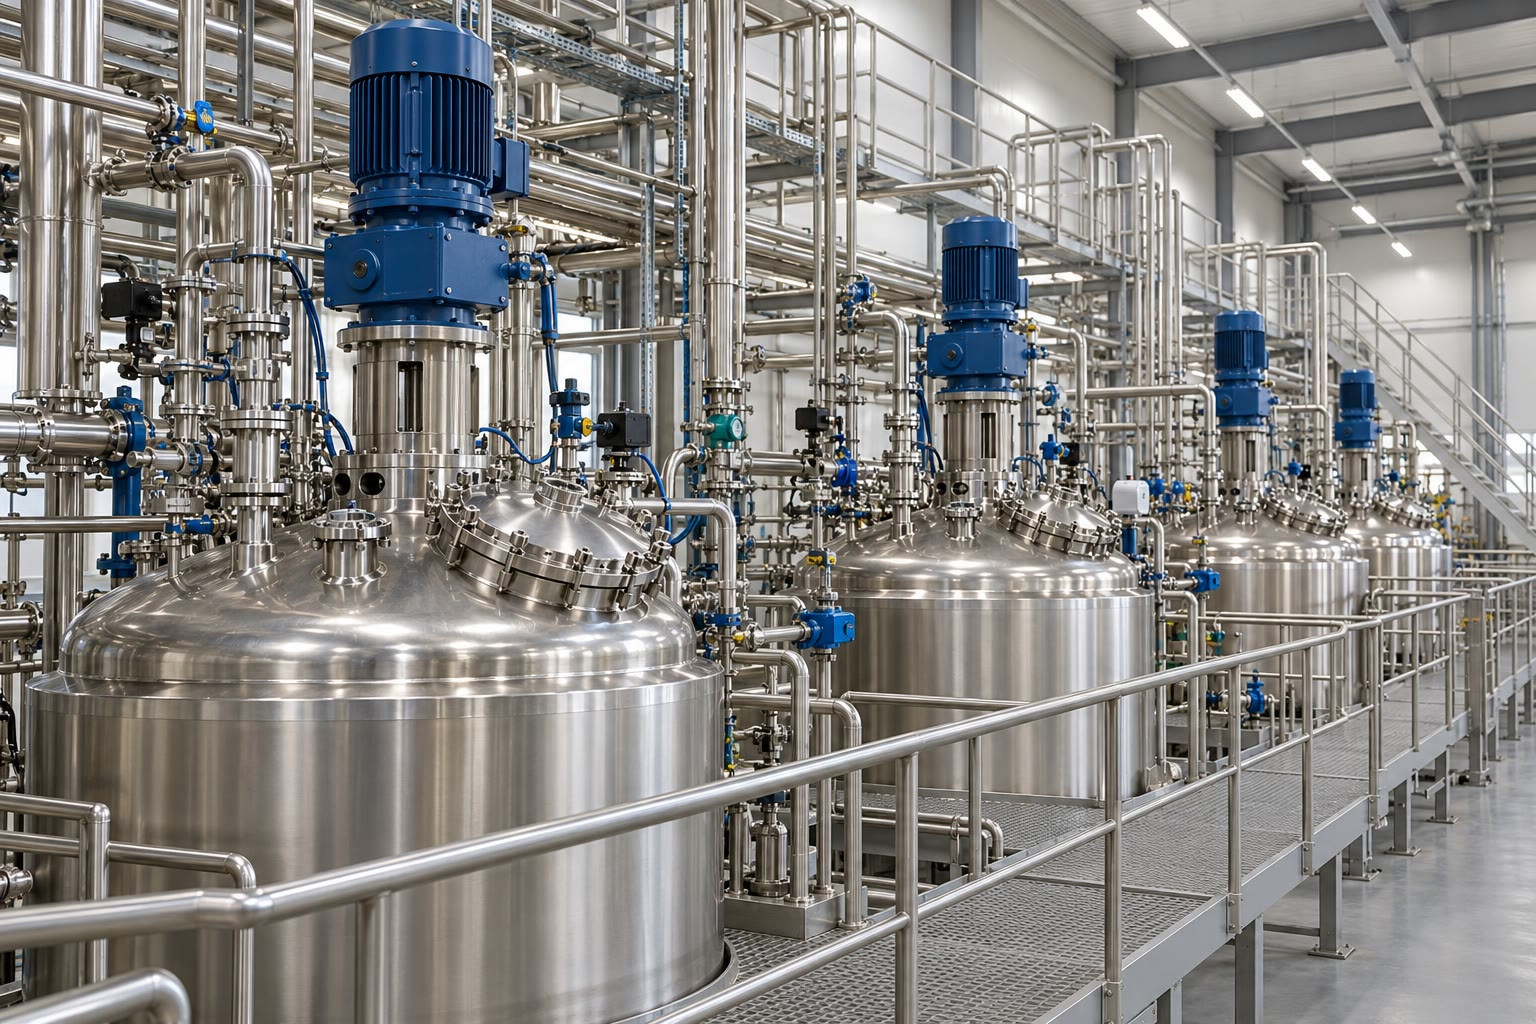
\includegraphics[width=0.6\linewidth]{images/book3/ai/b2-05-stirred-tanks.jpg}

{\small Reactores de tanque agitado en una planta química: cada recipiente lleva su
motor y su reductor, y el eje del agitador baja hasta la mezcla de reacción;
las tuberías traen las alimentaciones y se llevan el producto y el agua de refrigeración.}
\end{omfigure}

\section{Del reactor discontinuo al continuo}

\begin{definition}[Tipos de reactores]\label{def:b2:continuous-reactors:reactors}
Un \emph{reactor discontinuo}\index{reactor discontinuo} es un recipiente cerrado en el que la
reacción tiene lugar sin entrada ni salida de materia. Un
\emph{reactor continuo}\index{reactor continuo} está atravesado por un flujo estacionario
de materia. Dos reactores continuos ideales sirven de modelos:
\begin{itemize}
  \item el \emph{reactor continuo de tanque agitado}\index{reactor continuo de tanque agitado}
(RCTA), tan bien agitado que su contenido es
        uniforme y, por tanto, idéntico a la corriente que sale de él;
  \item el \emph{reactor de flujo pistón}\index{reactor de flujo piston@reactor de flujo pistón} (RFP), un tubo
        atravesado por el fluido sin mezcla a lo largo del flujo, en el que cada rebanada de
        fluido avanza como un pistón mientras reacciona.
\end{itemize}
\end{definition}

Se dice que un \omterm{def:b2:continuous-reactors:reactors}{reactor continuo} funciona en \emph{régimen estacionario} cuando
nada cambia en su interior con el tiempo: los caudales, las temperaturas y las
composiciones en cada punto son constantes. Se considera una sola reacción
$\mathrm A \to$ productos, con una alimentación líquida de densidad constante (de modo que el
caudal volumétrico $Q_v$ es el mismo a la entrada y a la salida) y
concentración $c_{A,0}$ a la entrada.

\begin{definition}[Tiempo de residencia]\label{def:b2:continuous-reactors:residence-time}
El \emph{tiempo de residencia}\index{tiempo de residencia} de un \omterm{def:b2:continuous-reactors:reactors}{reactor continuo} de
volumen $V$ alimentado con el caudal volumétrico $Q_v$ es $\tau = V/Q_v$: el tiempo
medio que un volumen de fluido pasa en su interior.
\end{definition}

\begin{definition}[Conversión]\label{def:b2:continuous-reactors:conversion}
La \emph{conversión}\index{conversion@conversión} del reactivo A es $X = (F_{A,0} -
F_A)/F_{A,0}$, donde $F_{A,0}$ y $F_A$ son los caudales molares de A que
entran en el reactor y salen de él; para un \omterm{def:b2:continuous-reactors:reactors}{reactor discontinuo}, $X = (n_{A,0} -
n_A)/n_{A,0}$. A densidad constante, $X = 1 - c_A/c_{A,0}$.
\end{definition}

La \omterm{def:b2:continuous-reactors:conversion}{conversión} se refiere a un reactivo, y a un reactor o a un paso; el grado de avance
final del volumen del primer año se refiere a una reacción y a su
reactivo limitante. Para una sola reacción cuyo reactivo limitante es A, ambos
coinciden.

\begin{proposition}[Reactor discontinuo]\label{prop:b2:continuous-reactors:batch}
En un \omterm{def:b2:continuous-reactors:reactors}{reactor discontinuo} de volumen constante, una reacción de primer orden alcanza la
\omterm{def:b2:continuous-reactors:conversion}{conversión} $X = 1 - \mathrm e^{-kt}$ al cabo del tiempo $t$, y una reacción de segundo
orden con concentraciones iniciales iguales $c_0$, la \omterm{def:b2:continuous-reactors:conversion}{conversión} $X =
kc_0t/(1 + kc_0t)$.
\end{proposition}

\begin{proof}
Son las leyes de velocidad integradas del volumen del primer año, $c_A = c_{A,0}
\mathrm e^{-kt}$ y $1/c_A = 1/c_{A,0} + kt$, escritas con $X = 1 -
c_A/c_{A,0}$.
\end{proof}

\section{El reactor continuo de tanque agitado}

\begin{omfigure}
\begin{tikzpicture}[font=\small, >={Stealth}]
  % batch
  \pic[transform shape] at (0,0) {rbflask={0.6}{omDef!20}};
  \node[below] at (0,-0.15) {discontinuo};
  % CSTR
  \begin{scope}[xshift=4.2cm]
    \draw[thick, fill=omDef!15] (-1.2,0) rectangle (1.2,2.4);
    \draw[thick] (0,3.0) -- (0,0.5);
    \draw[thick, fill=gray!40] (-0.5,0.45) rectangle (0.5,0.6);
    \draw[thick, fill=gray!30] (-0.25,3.0) rectangle (0.25,3.35);
    \draw[->, thick, omDef] (-2.8,2.0) -- (-1.2,2.0) node[pos=0.0, above, anchor=south west, inner sep=1pt] {$Q_v$, $c_{A,0}$};
    \draw[->, thick, omThm] (1.2,0.3) -- (2.5,0.3) node[pos=1, below] {$Q_v$, $c_A$};
    \node[fill=omDef!15, inner sep=1pt] at (0.62,1.5) {$V$, $c_A$};
    \node[below] at (0,-0.15) {tanque agitado};
  \end{scope}
  % PFR
  \begin{scope}[xshift=8.4cm, yshift=1.0cm]
    \draw[thick, fill=omDef!10] (0,0) rectangle (4.2,0.7);
    \fill[omThm!25] (2.0,0) rectangle (2.35,0.7);
    \draw[thick] (2.0,0) -- (2.0,0.7) (2.35,0) -- (2.35,0.7);
    \node[above] at (2.17,0.75) {$\dd V$};
    \draw[->, thick, omDef] (-0.9,0.35) -- (0,0.35) node[pos=0, above] {$F_{A,0}$};
    \draw[->, thick, omThm] (4.2,0.35) -- (5.0,0.35) node[pos=1, above] {$F_A$};
    \node[below] at (1.0,0) {$F_A(V)$};
    \node[below] at (2.1,-1.15) {tubo de flujo pistón};
  \end{scope}
\end{tikzpicture}

{\small Los tres reactores ideales. Un matraz discontinuo; un tanque agitado cuyo contenido
uniforme es el de la corriente de salida; un tubo recorrido en flujo pistón, en el
que el caudal de A disminuye de una rebanada a la siguiente.}
\end{omfigure}

\begin{proposition}[Balance de un tanque agitado]\label{prop:b2:continuous-reactors:cstr-balance}
En régimen estacionario, un tanque agitado de volumen $V$ en el que A desaparece a
la velocidad $r$ (mol por litro y por segundo) cumple
\[
  F_{A,0} - F_A - rV = 0, \qquad\text{es decir,}\qquad c_{A,0} - c_A = r\,\tau ,
\]
evaluándose la velocidad con la composición y la temperatura de salida.
\end{proposition}

\begin{proof}
Balance de A en el tanque durante $\dd t$: lo que entra, $F_{A,0}\dd t$,
menos lo que sale, $F_A\dd t$, menos lo que reacciona, $rV\dd t$, es igual a la
acumulación, nula en régimen estacionario. Como el tanque es uniforme, la velocidad es
la misma en todas partes e igual a la de la corriente de salida. Se divide por $Q_v$.
\end{proof}

\begin{theorem}[Conversión en un tanque agitado]\label{thm:b2:continuous-reactors:cstr}
Para una reacción de primer orden, $X = \dfrac{k\tau}{1 + k\tau}$; para una
reacción de segundo orden con concentraciones de alimentación iguales $c_0$ de los dos
reactivos, $X$ es la raíz en $[0, 1]$ de $Da\,(1 - X)^2 = X$, con $Da =
kc_0\tau$.
\end{theorem}

\begin{proof}
Orden 1: $r = kc_A$, luego $c_{A,0} - c_A = k\tau c_A$, $c_A = c_{A,0}/(1 + k\tau)$
y $X = 1 - 1/(1 + k\tau)$. Orden 2: $r = kc_A^2$ (las dos concentraciones siguen
siendo iguales), $c_0X = k\tau c_0^2(1 - X)^2$.
\end{proof}

El grupo adimensional $Da = k\tau$ (o $kc_0\tau$), el número de
Damköhler, compara el \omterm{def:b2:continuous-reactors:residence-time}{tiempo de residencia} con la escala de tiempo de la reacción:
él solo fija la \omterm{def:b2:continuous-reactors:conversion}{conversión}.

\begin{method}[Dimensionar un reactor]\label{met:b2:continuous-reactors:size-reactor}
\begin{enumerate}
  \item Escríbanse la ley de velocidad y la \omterm{def:b2:continuous-reactors:conversion}{conversión} exigida $X$.
  \item Con el balance del reactor elegido, hállese el número de Damköhler
        que da $X$.
  \item Dedúzcase $\tau$ de $Da$ y de la constante de velocidad a la temperatura de
        trabajo, y $V = \tau Q_v$ del caudal que hay que tratar.
\end{enumerate}
\end{method}

\section{El reactor de flujo pistón}

\begin{theorem}[Conversión en un reactor de flujo pistón]\label{thm:b2:continuous-reactors:pfr}
En régimen estacionario, el caudal de A a lo largo de un tubo de flujo pistón obedece
$\dd F_A/\dd V = -r$. Para una reacción de primer orden se obtiene $X = 1 -
\mathrm e^{-k\tau}$, y para una reacción de segundo orden con alimentaciones iguales, $X =
Da/(1 + Da)$: las leyes del \omterm{def:b2:continuous-reactors:reactors}{reactor discontinuo}, con el \omterm{def:b2:continuous-reactors:residence-time}{tiempo de residencia} en
lugar del tiempo.
\end{theorem}

\begin{proof}
Balance de A en la rebanada entre $V$ y $V + \dd V$: $F_A(V) - F_A(V + \dd V)
- r\,\dd V = 0$, de donde la ecuación diferencial. Con $F_A = Q_vc_A$ y
$\dd V = Q_v\,\dd t'$ (el tiempo $t'$ que una rebanada lleva en el tubo), se escribe
$\dd c_A/\dd t' = -r$: cada rebanada es un pequeño \omterm{def:b2:continuous-reactors:reactors}{reactor discontinuo} que permanece en el
tubo durante $\tau$. Separando las variables para $r = kc_A$ se obtiene $c_A = c_{A,0}
\mathrm e^{-k\tau}$ a la salida; para $r = kc_A^2$, $1/c_A - 1/c_0 = k\tau$.
\end{proof}

\begin{omfigure}
\begin{tikzpicture}
\begin{axis}[
  width=0.75\linewidth, height=6cm, xmin=0, xmax=10, ymin=0, ymax=1.05,
  axis x line=bottom, axis y line=left, xlabel={número de Damköhler $k\tau$},
  ylabel={conversión $X$}, tick label style={font=\small},
  label style={font=\small}, clip=false,
  legend style={font=\scriptsize, draw=none, at={(0.98,0.05)}, anchor=south east}]
\addplot[omThm, very thick] table[x=Da, y=pfr] {figdata/out/bachelor-2-reactors-a.dat};
\addplot[omProp, thick] table[x=Da, y=five] {figdata/out/bachelor-2-reactors-a.dat};
\addplot[omProp, thick, dashed] table[x=Da, y=two] {figdata/out/bachelor-2-reactors-a.dat};
\addplot[omDef, very thick] table[x=Da, y=cstr] {figdata/out/bachelor-2-reactors-a.dat};
\legend{flujo pistón, 5 tanques en serie, 2 tanques en serie, 1 tanque agitado}
\draw[dotted] (axis cs:2.303,0) -- (axis cs:2.303,0.9) -- (axis cs:9,0.9);
\fill[omThm] (axis cs:2.303,0.9) circle (1.4pt);
\fill[omDef] (axis cs:9,0.9) circle (1.4pt);
\end{axis}
\end{tikzpicture}

{\small \omterm{def:b2:continuous-reactors:conversion}{Conversión} de una reacción de primer orden en función de $k\tau$ en los reactores
ideales. Para un 90\,\% de \omterm{def:b2:continuous-reactors:conversion}{conversión}, un tubo de flujo pistón necesita $k\tau = \ln 10 = 2.3$,
y un solo tanque agitado $k\tau = 9$: cuatro veces el volumen. Los tanques en serie
se acercan al tubo.}
% (model curves, computed in figdata/bachelor-2/reactors.py)
\end{omfigure}

\begin{proposition}[Tanque o tubo]\label{prop:b2:continuous-reactors:compare}
Para cualquier velocidad que crezca con la concentración de A (cualquier orden
positivo), un \omterm{def:b2:continuous-reactors:reactors}{reactor de flujo pistón} alcanza una \omterm{def:b2:continuous-reactors:conversion}{conversión} dada con un volumen menor
que un tanque agitado.
\end{proposition}

\begin{proof}
Según los balances, $\tau_{\text{RCTA}} = c_{A,0}X/r(X)$ (la velocidad con la composición
de salida) y $\tau_{\text{RFP}} = c_{A,0}\int_0^X\dd X'/r(X')$. Como $r$
disminuye cuando $X$ aumenta, $1/r(X') \leq 1/r(X)$ en $[0, X]$, luego la
integral es como mucho $X/r(X)$. Gráficamente, en una representación de $1/r$ frente a $X$, el
$\tau$ del tubo es el área bajo la curva y el del tanque, el rectángulo de
altura $1/r(X)$ (figura siguiente). Para el orden 1: $\ln(1 + k\tau) \leq k\tau$, el
mismo enunciado en otra forma.
\end{proof}

El tanque agitado trabaja por completo a la concentración de salida, la más baja
del sistema, y por tanto a la velocidad más baja; el tubo aprovecha las concentraciones altas
cerca de su entrada. Las ventajas del tanque están en otra parte: una temperatura uniforme y fácil de controlar,
y un funcionamiento sencillo.

\begin{omfigure}
\begin{tikzpicture}
\begin{axis}[
  width=0.62\linewidth, height=5.6cm, xmin=0, xmax=1, ymin=0, ymax=22,
  axis x line=bottom, axis y line=left, xlabel={conversión $X$},
  ylabel={$1/r$ (unidades del modelo)}, tick label style={font=\small},
  label style={font=\small}, clip=false]
\fill[omDef!15] (axis cs:0,0) rectangle (axis cs:0.9,10);
\addplot[omThm, fill=omThm!20, draw=none, domain=0:0.9, samples=60] {1/(1-x)} \closedcycle;
\addplot[black, very thick] table[x=X, y=invr] {figdata/out/bachelor-2-reactors-c.dat};
\draw[omDef, thick] (axis cs:0,10) -- (axis cs:0.9,10) -- (axis cs:0.9,0);
\node[omDef, font=\scriptsize, anchor=south] at (axis cs:0.45,10.2) {tanque agitado: rectángulo, $\tau = 9$};
\node[omThm, font=\scriptsize, anchor=west] (pf) at (axis cs:0.05,6.5) {flujo pistón: área sombreada, $\tau = \ln 10$};
\draw[omThm, ->] (axis cs:0.25,6.0) -- (axis cs:0.3,0.8);
\end{axis}
\end{tikzpicture}

{\small Gráfico de Levenspiel de una reacción de primer orden ($k = 1$, $c_{A,0} = 1$).
Para un 90\,\% de \omterm{def:b2:continuous-reactors:conversion}{conversión} el tanque agitado necesita el rectángulo completo, y el flujo
pistón solo el área sombreada bajo la curva.}
% (model, computed in figdata/bachelor-2/reactors.py)
\end{omfigure}

\begin{proposition}[Tanques en serie]\label{prop:b2:continuous-reactors:cascade}
$N$ tanques agitados iguales en serie, de \omterm{def:b2:continuous-reactors:residence-time}{tiempo de residencia} total $\tau$, convierten una
reacción de primer orden hasta $X_N = 1 - (1 + k\tau/N)^{-N}$, que aumenta con
$N$ y tiende al valor del flujo pistón, $1 - \mathrm e^{-k\tau}$.
\end{proposition}

\begin{proof}
Cada tanque divide la concentración por $1 + k\tau/N$. Y $(1 +
k\tau/N)^{-N} = \exp[-N\ln(1 + k\tau/N)] \to \mathrm e^{-k\tau}$, ya que
$N\ln(1 + u/N) \to u$.
\end{proof}

\begin{definition}[Selectividad]\label{def:b2:continuous-reactors:selectivity}
Cuando un reactivo puede dar varios productos, la \emph{selectividad}\index{selectividad}
hacia el producto deseado B es la cantidad de B formada dividida por la cantidad del
reactivo consumida (multiplicada por la razón estequiométrica): dice qué parte de
lo que reaccionó fue por el buen camino.
\end{definition}

\begin{proposition}[Un intermedio en un tanque y en un tubo]\label{prop:b2:continuous-reactors:consecutive}
Para reacciones consecutivas de primer orden $\mathrm A \xrightarrow{k_1} \mathrm B
\xrightarrow{k_2} \mathrm C$, con una alimentación de A sola, la concentración de B
a la salida es máxima para $\tau = \ln(k_2/k_1)/(k_2 - k_1)$ en un
\omterm{def:b2:continuous-reactors:reactors}{reactor de flujo pistón} y para $\tau = 1/\sqrt{k_1k_2}$ en un tanque agitado; el
máximo es más alto en el tubo.
\end{proposition}

\begin{proof}
Tubo: con las leyes del \omterm{def:b2:continuous-reactors:reactors}{reactor discontinuo} (volumen del primer año) se obtiene $c_B = c_{A,0}\frac{k_1}{k_2 - k_1}
(\mathrm e^{-k_1\tau} - \mathrm e^{-k_2\tau})$, máxima donde la derivada
se anula, $k_1\mathrm e^{-k_1\tau} = k_2\mathrm e^{-k_2\tau}$. Tanque: $c_A =
c_{A,0}/(1 + k_1\tau)$ y el balance de B, $c_B = k_1\tau c_A - k_2\tau c_B$,
da $c_B = c_{A,0}k_1\tau/[(1 + k_1\tau)(1 + k_2\tau)]$, cuya derivada
se anula cuando $k_1k_2\tau^2 = 1$. La comparación de los máximos es el
\cref{exo:b2:continuous-reactors:10}.
\end{proof}

\section{Balance térmico y seguridad}

\begin{definition}[Aumento adiabático de temperatura]\label{def:b2:continuous-reactors:adiabatic-rise}
El \emph{aumento adiabático de temperatura}\index{aumento adiabatico de temperatura@aumento adiabático de temperatura}
$\Delta T_{\text{ad}}$ de una mezcla de reacción es el aumento de temperatura que
experimentaría si la reacción fuera completa y no se evacuara nada de calor.
\end{definition}

\begin{proposition}[Aumento adiabático de una mezcla líquida]\label{prop:b2:continuous-reactors:adiabatic}
Para una mezcla de densidad $\rho$ y capacidad calorífica másica $c_p$, en la que
el reactivo A, a la concentración $c_{A,0}$, reacciona con la entalpía
$\Delta_r H$ por mol de A, el aumento de temperatura a la \omterm{def:b2:continuous-reactors:conversion}{conversión} $X$ sin
pérdida de calor es
\[
  \Delta T = \frac{(-\Delta_r H)\,c_{A,0}\,X}{\rho\,c_p}, \qquad
  \Delta T_{\text{ad}} = \frac{(-\Delta_r H)\,c_{A,0}}{\rho\,c_p} .
\]
\end{proposition}

\begin{proof}
Por unidad de volumen, el calor liberado, $(-\Delta_r H)c_{A,0}X$, calienta una
masa $\rho$ de capacidad calorífica $c_p$ (primer principio a presión constante, las dos
etapas de la \cref{prop:b2:reaction-enthalpy:flame}).
\end{proof}

Una mezcla diluida es segura: unos pocos grados de aumento. Una mezcla concentrada y fuertemente
\omterm{def:b2:reaction-enthalpy:exothermic}{exotérmica} puede calentarse a sí misma cientos de kelvin, lo bastante para hacer hervir el
disolvente o desencadenar otra reacción. Y la velocidad crece exponencialmente con la
temperatura: el calor acelera la reacción, que libera calor más deprisa.

\begin{proposition}[Estados estacionarios de un tanque agitado refrigerado]\label{prop:b2:continuous-reactors:steady-states}
Para un tanque agitado con alimentación a $T_0$, refrigerado por una camisa a $T_0$ con un
coeficiente de transmisión de calor por área $UA$, las temperaturas estacionarias posibles
$T$ son las soluciones de
\[
  \underbrace{\Delta T_{\text{ad}}\,X(T)}_{\text{calor generado}} =
  \underbrace{(1 + \kappa)(T - T_0)}_{\text{calor evacuado}}, \qquad
  \kappa = \frac{UA}{Q_v\rho c_p},
\]
donde $X(T) = k(T)\tau/(1 + k(T)\tau)$ para una reacción de primer orden. La generación es
una curva en S de $T$, y la evacuación una recta: puede haber una o tres
intersecciones.
\end{proposition}

\begin{proof}
Balance de energía del tanque en régimen estacionario, por unidad de tiempo: el calor
liberado por la reacción, $(-\Delta_r H)F_{A,0}X$, sale con la corriente de
salida, que se calienta de $T_0$ a $T$, $Q_v\rho c_p(T - T_0)$, y a través de
la camisa, $UA(T - T_0)$. Se divide por $Q_v\rho c_p$. Con la ley de Arrhenius,
$X(T)$ pasa de 0 a 1 en un intervalo estrecho de temperatura: una S.
\end{proof}

\begin{omfigure}
\begin{tikzpicture}
\begin{axis}[
  width=0.75\linewidth, height=6.2cm, xmin=300, xmax=470, ymin=0, ymax=250,
  axis x line=bottom, axis y line=left, xlabel={temperatura del tanque $T$ (K)},
  ylabel={calor por unidad de caudal (K)}, tick label style={font=\small},
  label style={font=\small}, clip=true]
\addplot[omThm, very thick] table[x=T, y=gen] {figdata/out/bachelor-2-reactors-b.dat};
\addplot[omDef, very thick] table[x=T, y=rem] {figdata/out/bachelor-2-reactors-b.dat};
\fill[black] (axis cs:300.03,0.04) circle (2pt);
\fill[white, draw=black] (axis cs:390.4,135.6) circle (2pt);
\fill[black] (axis cs:429.6,194.4) circle (2pt);
\node[font=\scriptsize, anchor=north west, fill=white, inner sep=1pt] at (axis cs:318,58) {frío, estable}; \draw[black!60] (axis cs:301.5,2) -- (axis cs:318,52);
\node[font=\scriptsize, anchor=north west] at (axis cs:393,132) {inestable};
\node[font=\scriptsize, anchor=south east] at (axis cs:426,197) {caliente, estable};
\node[omThm, font=\scriptsize, anchor=north west] at (axis cs:440,196) {generado};
\node[omDef, font=\scriptsize, anchor=south east] at (axis cs:452,232) {evacuado};
\end{axis}
\end{tikzpicture}

{\small Diagrama de Semenov de un tanque agitado refrigerado (parámetros del modelo). El
calor generado (rojo) y el calor evacuado (recta azul) se cortan tres veces. El
estado intermedio es inestable: un poco más caliente y gana la generación, el tanque
se embala hacia el estado caliente; un poco más frío y vuelve al estado
frío.}
% (model, computed in figdata/bachelor-2/reactors.py)
\end{omfigure}

La estabilidad de cada estado se deduce de las pendientes: en una intersección
donde la recta de evacuación es más pendiente que la curva de generación, un pequeño aumento de
temperatura evacua más calor del que genera, y el tanque vuelve a enfriarse;
donde la curva de generación es más pendiente, un pequeño aumento se alimenta a sí mismo. (El
análisis riguroso linealiza los balances dependientes del tiempo; aquí se
admite.)

\begin{definition}[Embalamiento térmico]\label{def:b2:continuous-reactors:runaway}
Un \emph{embalamiento térmico}\index{embalamiento termico@embalamiento térmico} es el aumento autoacelerado
de la temperatura de una mezcla en reacción cuya generación de calor, que crece
exponencialmente con la temperatura, supera la evacuación de calor.
\end{definition}

\begin{method}[Balance térmico de un reactor]\label{met:b2:continuous-reactors:heat-balance}
\begin{enumerate}
  \item Calcúlese el \omterm{def:b2:continuous-reactors:adiabatic-rise}{aumento adiabático de temperatura}: si es de unos pocos kelvin, el
        reactor es térmicamente seguro.
  \item En caso contrario, calcúlese la potencia de refrigeración, $(-\Delta_r H)F_{A,0}X$ menos el
        calor que se lleva la corriente de salida, y compruébese que la camisa o el serpentín
        pueden evacuarla.
  \item Compruébese la estabilidad del punto de funcionamiento (pendientes en un diagrama
        de Semenov) y qué ocurriría si fallara la refrigeración: la
        temperatura máxima alcanzada, $T + \Delta T_{\text{ad}}(1 - X)$ para
        el reactivo aún presente.
\end{enumerate}
\end{method}

\section{Del protocolo a la planta}

Una síntesis que funciona en un matraz de \qty{1}{L} no se escala sin más
mil veces. El volumen, y el calor liberado, crecen como el cubo del
tamaño; la pared, por la que sale el calor, como su cuadrado. Un recipiente diez
veces más ancho tiene mil veces el volumen pero solo cien veces la
superficie de refrigeración: una reacción que se mantenía templada en el matraz puede embalarse en
el tanque. La práctica industrial añade por ello el reactivo más reactivo
lentamente (la reacción no puede liberar más calor del que aporta el reactivo alimentado), diluye,
refrigera con serpentines internos o pasa a \omterm{def:b2:continuous-reactors:reactors}{reactores continuos} de pequeño volumen,
cuya pequeña retención limita lo que puede salir mal.

La \omterm{def:b2:continuous-reactors:selectivity}{selectividad} es la otra preocupación. Una planta no tira lo que no ha
reaccionado: separa el producto y recicla los reactivos, como en el
bucle del amoníaco. Puede, por tanto, aceptar una \omterm{def:b2:equilibrium-shifts:single-pass}{conversión por paso} modesta si la
\omterm{def:b2:continuous-reactors:selectivity}{selectividad} es alta, ya que todo subproducto es materia prima perdida y residuo que
tratar.

\begin{inthelab}[Un tanque agitado en la mesa de laboratorio]
La cinética de una reacción destinada a una planta continua se mide en un
pequeño reactor agitado alimentado por dos bombas calibradas, con una célula de conductividad
o un espectrómetro en línea a la salida. Al variar el caudal varía $\tau$;
la concentración estacionaria de salida para cada $\tau$ da directamente la velocidad, por el
balance $r = (c_{A,0} - c_A)/\tau$, sin ninguna integración.
\end{inthelab}

\section{Ejercicios}

\begin{exercise}[$\star$]\label{exo:b2:continuous-reactors:1}
Un tanque agitado de \qty{2.0}{m^3} se alimenta a \qty{0.50}{L/s}. Calcúlese su
\omterm{def:b2:continuous-reactors:residence-time}{tiempo de residencia} en segundos y en horas.
\end{exercise}

\begin{exercise}[$\star$]\label{exo:b2:continuous-reactors:2}
Una reacción de primer orden tiene $k = \qty{1.2e-3}{s^{-1}}$ a la temperatura de
trabajo. Calcúlese la \omterm{def:b2:continuous-reactors:conversion}{conversión} en un tanque agitado y en un tubo de flujo pistón
del mismo \omterm{def:b2:continuous-reactors:residence-time}{tiempo de residencia}, \qty{30}{min}.
\end{exercise}

\begin{exercise}[$\star$]\label{exo:b2:continuous-reactors:3}
¿Qué \omterm{def:b2:continuous-reactors:residence-time}{tiempo de residencia} en flujo pistón da un 99\,\% de \omterm{def:b2:continuous-reactors:conversion}{conversión} de una reacción de primer
orden con $k = \qty{0.020}{s^{-1}}$? ¿Y en un tanque agitado?
\end{exercise}

\begin{exercise}[$\star$]\label{exo:b2:continuous-reactors:4}
Una disolución acuosa de \qty{0.50}{mol/L} de un reactivo cuya reacción
libera \qty{-120}{kJ/mol} ($\rho = \qty{1.0}{kg/L}$, $c_p =
\qty{4.2}{J/(g.K)}$) reacciona por completo. Calcúlese el \omterm{def:b2:continuous-reactors:adiabatic-rise}{aumento adiabático de
temperatura}. ¿Es peligroso un fallo de la refrigeración?
\end{exercise}

\begin{exercise}[$\star\star$]\label{exo:b2:continuous-reactors:5}
Para una reacción de segundo orden con alimentaciones iguales ($kc_0 = \qty{0.010}{s^{-1}}$),
calcúlese el \omterm{def:b2:continuous-reactors:residence-time}{tiempo de residencia} para un 80\,\% de \omterm{def:b2:continuous-reactors:conversion}{conversión} en un tanque agitado y en un
tubo de flujo pistón. Compárese la razón con la de una reacción de primer orden.
\end{exercise}

\begin{exercise}[$\star\star$]\label{exo:b2:continuous-reactors:6}
Tres tanques agitados iguales en serie, de \omterm{def:b2:continuous-reactors:residence-time}{tiempo de residencia} total \qty{10}{min},
tratan una reacción de primer orden con $k = \qty{0.50}{min^{-1}}$. Calcúlese la
\omterm{def:b2:continuous-reactors:conversion}{conversión} y compárese con un solo tanque y con un tubo del mismo \omterm{def:b2:continuous-reactors:residence-time}{tiempo de residencia}
total.
\end{exercise}

\begin{exercise}[$\star\star$]\label{exo:b2:continuous-reactors:7}
Un tanque agitado convierte el 70\,\% de un reactivo (primer orden). Se duplica el caudal.
¿Cuál es la nueva \omterm{def:b2:continuous-reactors:conversion}{conversión}? ¿En qué factor debe aumentar el volumen para
recuperar el 70\,\%?
\end{exercise}

\begin{exercise}[$\star\star$]\label{exo:b2:continuous-reactors:8}
Un tanque de \qty{5.0}{m^3} trabaja a \qty{350}{K} con una alimentación de
\qty{2.0}{mol/L} de reactivo a \qty{1.0}{L/s}, convertido en un 90\,\%, $\Delta_r H
= \qty{-80}{kJ/mol}$, $\rho c_p = \qty{4.0}{kJ/(L.K)}$, alimentación a \qty{330}{K}.
Calcúlense el calor liberado por segundo, el calor que se lleva la corriente de
salida y la potencia de refrigeración de la camisa.
\end{exercise}

\begin{exercise}[$\star\star$]\label{exo:b2:continuous-reactors:9}
Un matraz de \qty{1.0}{L} y un reactor de \qty{1.0}{m^3} tienen la misma forma.
¿Por qué factor quedan multiplicados el volumen, el área de la pared y la razón entre ambos?
Explíquese por qué una reacción fácil de refrigerar en el matraz puede
embalarse en el reactor.
\end{exercise}

\begin{exercise}[$\star\star\star$]\label{exo:b2:continuous-reactors:10}
Para $\mathrm A \to \mathrm B \to \mathrm C$ con $k_1 = \qty{0.10}{min^{-1}}$
y $k_2 = \qty{0.050}{min^{-1}}$, calcúlense el \omterm{def:b2:continuous-reactors:residence-time}{tiempo de residencia} óptimo y el
rendimiento máximo en B en un \omterm{def:b2:continuous-reactors:reactors}{reactor de flujo pistón} y en un tanque agitado, y explíquese
por qué el tubo funciona mejor para un intermedio.
\end{exercise}

\begin{exercise}[$\star\star\star$]\label{exo:b2:continuous-reactors:11}
Con el diagrama de Semenov del capítulo, descríbase qué ocurre cuando se eleva
lentamente la temperatura del refrigerante y luego se vuelve a bajar lentamente: demuéstrese que
el tanque salta de la rama fría a la caliente a una temperatura y vuelve a
otra (histéresis).
\end{exercise}

\begin{exercise}[$\star\star\star$]\label{exo:b2:continuous-reactors:12}
Se carga un \omterm{def:b2:continuous-reactors:reactors}{reactor discontinuo} con \qty{2.0}{mol/L} de reactivo ($\Delta_r H =
\qty{-100}{kJ/mol}$, $\rho c_p = \qty{4.0}{kJ/(L.K)}$) y se calienta hasta la
temperatura de trabajo. La refrigeración falla entonces al 25\,\% de \omterm{def:b2:continuous-reactors:conversion}{conversión}. Calcúlese la
temperatura que puede alcanzar la mezcla. En una operación semicontinua, el mismo
reactivo se añade lentamente y se consume a medida que llega, de modo que como mucho un 5\,\%
de la carga está presente sin reaccionar: ¿cuál es ahora el aumento en el peor caso?
\end{exercise}

\section{Problema: jabón en un tanque}

\begin{problem}[{Problema de fin de semana --- la saponificación de un éster en un
tanque agitado: cinética, dimensionado para un 90\,\% de conversión, las alternativas de un
tubo y de una cascada, y el balance térmico}]
\label{pb:b2:continuous-reactors:1}
El etanoato de etilo se saponifica con hidróxido de sodio,
\ce{CH3COOC2H5 + OH- -> CH3COO- + C2H5OH}, una reacción de segundo orden (de primer
orden respecto de cada reactivo). Una planta trata \qty{0.50}{L/s} de una mezcla cuyas
concentraciones de éster y de hidróxido a la entrada son ambas $c_0 =
\qty{0.10}{mol/L}$. En este problema se toma $k = \qty{0.11}{L/(mol.s)}$ a la
temperatura de trabajo y $\Delta_r H = \qty{-55}{kJ/mol}$ (valores fijados para el
ejercicio); la mezcla tiene la densidad y la capacidad calorífica del agua,
$\rho = \qty{997}{kg/m^3}$, $c_p = \qty{4.18}{kJ/(kg.K)}$.

\medskip
\noindent\textbf{Parte I --- Cinética.}
\begin{enumerate}
  \item Escríbase la ley de velocidad. ¿Por qué siguen siendo iguales las dos concentraciones?
  \item En un matraz discontinuo, ¿cuánto tarda un 90\,\% de \omterm{def:b2:continuous-reactors:conversion}{conversión}?
  \item Calcúlese el tiempo de semirreacción en el matraz. ¿Por qué depende de $c_0$?
  \item Escríbase el número de Damköhler de la reacción para un \omterm{def:b2:continuous-reactors:residence-time}{tiempo de residencia} $\tau$.
\end{enumerate}

\medskip
\noindent\textbf{Parte II --- Un solo tanque agitado.}
\begin{enumerate}[resume]
  \item Escríbase el balance de éster en el tanque en régimen estacionario.
  \item Demuéstrese que $Da\,(1 - X)^2 = X$.
  \item Calcúlese el número de Damköhler necesario para $X = 0.90$.
  \item Calcúlese el \omterm{def:b2:continuous-reactors:residence-time}{tiempo de residencia}.
  \item Calcúlese el volumen del tanque.
  \item ¿Qué concentración ``ve'' la reacción en todo el tanque,
        y por qué es tan grande el tanque?
\end{enumerate}

\medskip
\noindent\textbf{Parte III --- Un tubo, una cascada.}
\begin{enumerate}[resume]
  \item Calcúlense el número de Damköhler y el volumen de un tubo de flujo pistón para
        la misma tarea.
  \item Calcúlese la razón de los dos volúmenes.
  \item Tres tanques iguales en serie: escríbase la relación entre las concentraciones
        de salida de dos tanques sucesivos.
  \item El volumen total de los tres tanques que da un 90\,\% es de
        \qty{0.85}{m^3}. Compruébese calculando la concentración que sale de cada
        tanque.
  \item ¿Qué disposición se construiría, y por qué podría preferirse aun así un solo
        tanque?
\end{enumerate}

\medskip
\noindent\textbf{Parte IV --- El calor.}
\begin{enumerate}[resume]
  \item Calcúlese el \omterm{def:b2:continuous-reactors:adiabatic-rise}{aumento adiabático de temperatura} de la mezcla.
  \item Calcúlese el calor liberado por segundo en el tanque.
  \item ¿Hace falta refrigerar? ¿Es posible un embalamiento?
  \item ¿Qué cambiaría con una mezcla alimentada a \qty{2.0}{mol/L}?
  \item Calcúlese la masa de etanoato de sodio producida al día.
  \item Si la reacción se lleva a cabo a una temperatura más alta, ¿cómo cambia el volumen
        del tanque, y cuál es el coste?
  \item Indíquese el volumen del tanque agitado único que convierte el 90\,\% del
        éster con esta alimentación.
\end{enumerate}
\end{problem}
